\documentclass[10pt,conference]{IEEEtran}
\usepackage[utf8]{inputenc}
\usepackage{amsmath}
\usepackage{amsfonts}
\usepackage{amssymb}
\usepackage{graphicx}
\usepackage{cleveref}
\usepackage{relsize}

\newcommand{\ie}{i.e.\ }
\newcommand{\eg}{e.g.\ }
\crefname{section}{\S}{\S\S}
\crefname{subsection}{\S}{\S\S}
\crefname{subsubsection}{\S}{\S\S}

%% MATHS
\newcommand{\round}{\mathrm{Round}}
\newcommand{\pfp}{+_{\mathrm{fp}}}
\newcommand{\absv}[1]{\vert #1\vert}
\newcommand{\Pro}{\mathbb{P}}
\newcommand{\F}{\mathbb{F}}
\newcommand{\R}{\mathbb{R}}
\newcommand{\ceil}[1]{\lceil #1 \rceil}
\newcommand{\floor}[1]{\lfloor #1 \rfloor}
\newcommand{\intvl}[1]{\mathlarger{\left[\right.}  #1 \mathlarger{\left.\right]}}
\newcommand{\inv}{^{-1}}
\newcommand{\fintvl}[1][x]{\mathlarger{\lfloor}#1,#1\mathlarger{\rceil}}


\title{A probabilistic approach to the accuracy and stability of numerical algorithms}
\author{George Constantinides and Fredrik Dahlqvist \\ Department of Electrical and Electronic Engineering\\ Imperial College London}
\begin{document}
\maketitle

\begin{abstract}

\end{abstract}

\section{Introduction}
\begin{itemize}
\item Traditional approach to accuracy and stability: worst-case analysis
\item We are interested analysis of \emph{typical} behaviour. This can be made precise by using probabilities: \eg accuracy and stability guarantees in 99\% of executions
\item Recent probabilistic approaches to numerical accuracy (Nick Higham, Ilse Ipsen) focus on large/high-dimensional problems and rely on concentration of measure inequalities which provide useful information in this context.
\item Our approach is exact (no concentration of measure inequalities) but tailored to smaller programs. 
\item Test-cases: `small' scalar products for accuracy and ray tracing algorithm (Slabs method) for stability. 
\end{itemize} 

\section{A probabilistic model of rounding errors}

\subsection{Rounding error distribution}\label{subsec:error_dist}

\begin{itemize}
\item Compute the distribution of the random variable $\frac{X-\round(X)}{X}$ given the random variable $X$
\item Show that under mild assumptions on the distribution of $X$, the distribution of rounding errors is given by the roughly trapezoidal distribution of Fig \ref{fig:trapeze}.
\begin{figure}[ht!]
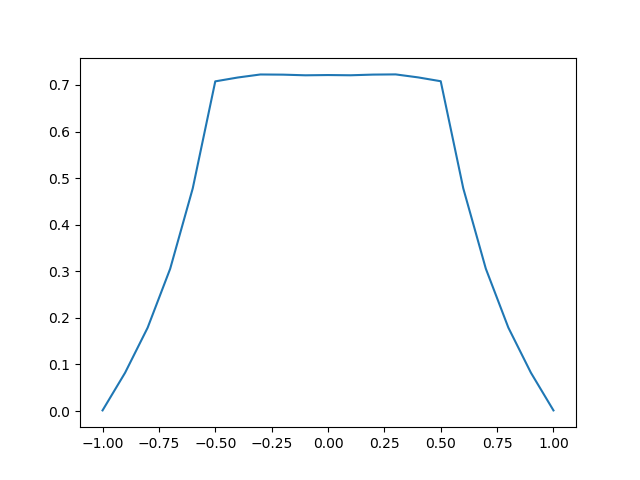
\includegraphics[scale=0.55]{trapeze_dist}
\caption{Typical distribution of rounding errors (in unit roundoffs)}
\label{fig:trapeze}
\end{figure}
\end{itemize}


\subsubsection{Derivation of the rounding error distribution}
Suppose a continuous (real-valued) random variable $X$ is distributed according to a probability density function $f$ (for example $X$ could model a stochastic, analog input signal), we can explicitly compute the distribution of the relative error induced by the quantization procedure (for example when the analog signal is digitized). We will `normalize' the result by working in units of $u$, the unit roundoff. Since the relative rounding error lies in the interval $[-u,u]$, the normalized relative error will lie in the interval $[-1,1]$.  We start by looking at the cumulative distribution function, \ie we compute the function:
\begin{align*}
c(t):=\Pro\left(\frac{X-\round(X)}{X}\leq tu\right)
\end{align*}
where $u$ is the unit roundoff. Clearly $\round(X)$ can take any value in $\F$, and given $x\in\F$ it is only possible to have $\round(X)=x$ if $X\in \left[\floor{x},\ceil{x}\right[$. This partitions $\R$

\subsection{Probabilistic version of the IEEE 754 standard}\label{subsec:prob_ieee754}

\begin{itemize}
\item Replace the usual non-deterministic 
\[
x\pfp y=(x+y)(1+\varepsilon), \absv{\varepsilon}\leq u
\]
with
\[
x\pfp y=(x+y)(1+\varepsilon)
\]
where $\varepsilon$ is a random variable of known distribution.
\item The `typical' distribution of $\varepsilon$ is described in \cref{subsec:error_dist}.
\end{itemize}

\section{Rounding error distribution of simple programs}

\subsection{Probabilistic programs}
\begin{itemize}
\item What they are: (1) programs which can sample from known probability distributions, (2) Programs whose inputs can be probabilistic.
\item The probabilistic model of IEEE 754 of \cref{subsec:prob_ieee754} turns any deterministic program into a probabilistic one.
\end{itemize}

\subsection{How probabilistic programs process probabilistic inputs}
\begin{itemize}
\item Pushing a distribution through a deterministic function
\item Pushing a distribution through a probabilistic function
\item Pushing a distribution through an \texttt{if then else} statement
\item Pushing a distribution through a simple program
\item Application to programs with probabilistic rounding errors (\cref{subsec:prob_ieee754})
\end{itemize}

\section{Probabilistic accuracy and stability}

\subsection{Accuracy: scalar products}

\begin{itemize}
\item Probabilistic accuracy
\item Comparison with classical worst-case analysis (\cite[3.1]{higham2002accuracy})
\end{itemize}

\subsection{Stability: ray tracing via the slabs method}

\bibliographystyle{plain}
\bibliography{bib/constantinides-dahlqvist}

\end{document}